\documentclass[aspectratio=169,unicode,dvipdfmx,14pt]{beamer}

\usepackage{url}
\usepackage{bm}
\usepackage{amsmath}
\usepackage{amssymb}
\usepackage{graphicx}
\usepackage[absolute,overlay]{textpos}
\usepackage{hyperref}
\usepackage{listings}

\usefonttheme[onlymath]{serif}

\DeclareMathOperator*{\argmax}{argmax}

\hypersetup{
	setpagesize=false,
	bookmarksnumbered=true,%
	bookmarksopen=true,%
	colorlinks=true,%
	linkcolor=blue,
	citecolor=red,
}

\newcommand\FontMath{\fontsize{10}{12}\selectfont}
\renewcommand{\baselinestretch}{1.3}
\renewcommand{\familydefault}{\sfdefault}
\renewcommand{\kanjifamilydefault}{\gtdefault}
\usepackage[deluxe, expert]{otf}

\setbeamertemplate{navigation symbols}{}
\setbeamertemplate{footline}[frame number]
\setbeamerfont{footline}{size={\fontsize{15}{15}}}

\setbeamerfont{author}{size=\Large}
\setbeamerfont{institute}{size=\normalsize\itshape}
\setbeamerfont{title}{size=\huge}
\setbeamerfont{subtitle}{size=\LARGE\normalfont\slshape}


\title{\ \\正規分布}
\author{正田 備也\\{\small masada@rikkyo.ac.jp}}
\date{}

\begin{document}

\begin{frame}
\titlepage
\end{frame}

\section{単変量正規分布}

\begin{frame}\frametitle{Contents}
\Large \tableofcontents[currentsection]
\end{frame}

\begin{frame}{正規分布 normal distribution}
\begin{itemize}
\item ガウス分布 Gaussian distributionとも呼ばれる
\item 連続量をモデル化するときによく使われる
\begin{itemize}
\item 下図は2変量正規分布の確率密度関数の例:
\end{itemize}
\end{itemize}
\begin{figure}
\center
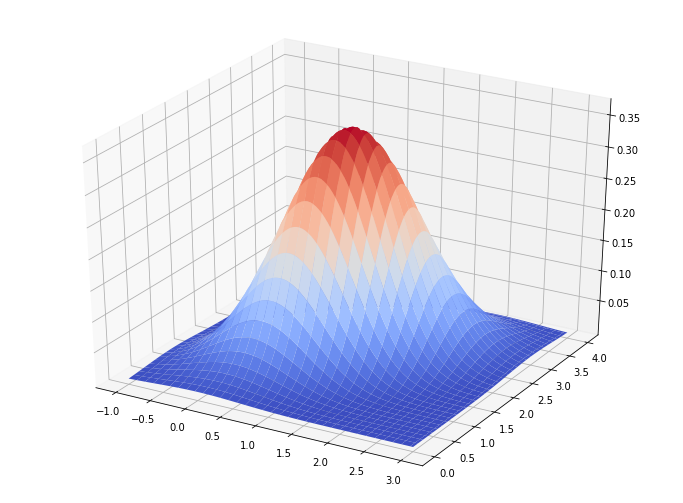
\includegraphics[scale=0.3]{normal_distribution_1.png}
\end{figure}
\end{frame}

\begin{frame}{単変量正規分布}
\begin{itemize}
\item 単変量正規分布は、$\mathbb{R}=(-\infty,\infty)$上に定義される
\item 単変量正規分布のパラメータは、平均$\mu$と標準偏差$\sigma$
\begin{itemize}
\item 平均$\mu$、標準偏差$\sigma$の単変量正規分布を、以下$\mathcal{N}(\mu,\sigma^2)$と書く
\item 確率変数$x$が$\mathcal{N}(\mu,\sigma^2)$に従うことを、以下$x\sim\mathcal{N}(\mu,\sigma^2)$と書く
\end{itemize}
\item 単変量正規分布$x\sim\mathcal{N}(\mu,\sigma^2)$の確率密度関数pdfは:
\begin{align}
p(x;\mu,\sigma) = \frac{1}{\sqrt{2\pi\sigma^2}}\exp\Big( - \frac{(x - \mu)^2}{2\sigma^2} \Big)
\end{align}
\begin{itemize}
\item 「;」は、その右側にある$\mu$と$\sigma$が自由パラメータ(我々が値を指定する必要があるパラメータ)であることを意味する
\end{itemize}
\end{itemize}
\end{frame}

\begin{frame}{参考:ガウス積分}
\begin{itemize}
\item $\frac{1}{\sqrt{2\pi\sigma^2}}$って、何?
\begin{itemize}
\item $-\infty$から$\infty$までの範囲で積分すると1になるようにするには、この値を掛け算しておかないといけない、という意味
\item ひとことで言えば、規格化定数
\end{itemize}
\item 逆に言えば、$\int_{-\infty}^\infty \exp\Big( - \frac{(x - \mu)^2}{2\sigma^2} \Big) dx = \sqrt{2\pi\sigma^2}$が成り立つ、ということ
\begin{itemize}
\item こういう積分を、ガウス積分と呼ぶ
\item ガウス積分の公式:$\int_{-\infty}^\infty e^{-a(x+b)^2}dx = \sqrt{\frac{\pi}{a}}$
\end{itemize}
\end{itemize}
\end{frame}


\begin{frame}{密度関数についての注意事項}
\begin{align}
p(x;\mu,\sigma) = \frac{1}{\sqrt{2\pi\sigma^2}}\exp\Big( - \frac{(x - \mu)^2}{2\sigma^2} \Big)
\end{align}
\begin{itemize}
\item 密度関数の$x$に特定の値を代入して得られる値は、確率としての意味を持たない
\begin{itemize}
\item そもそも、密度関数の値は1を超えることがいくらでもある
\end{itemize}
\item 密度関数を特定の範囲で積分すると、確率とみなすことのできる値が得られる
\begin{itemize}
\item 当然、全範囲で積分すると1になる(つまり$\int_{-\infty}^\infty p(x;\mu,\sigma)dx = 1$)
\end{itemize}
\end{itemize}
\end{frame}

\begin{frame}{単変量正規分布の密度関数の例}
\begin{figure}[b]
\begin{center}
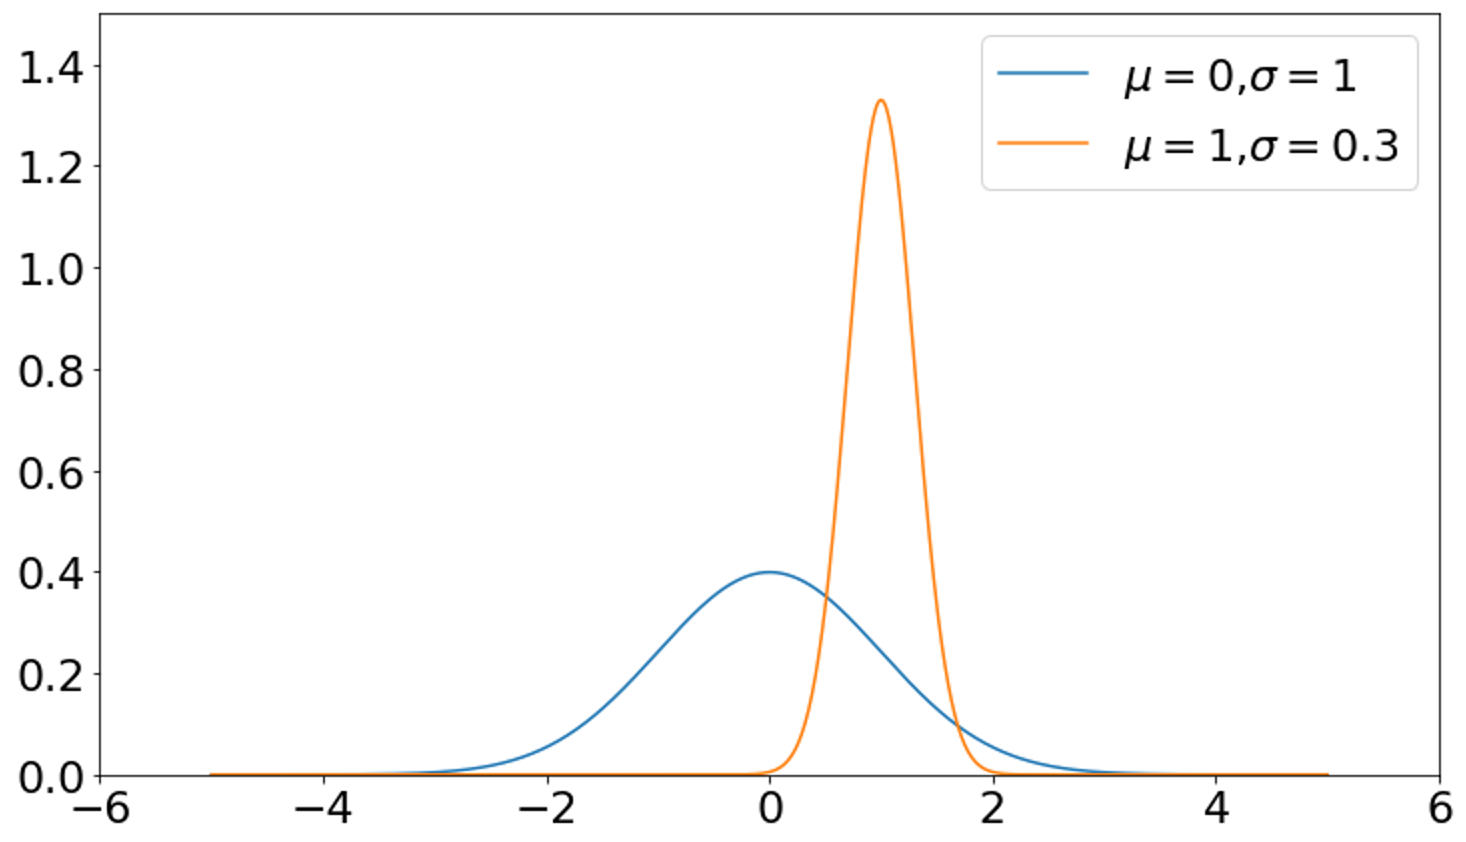
\includegraphics[scale=0.45]{normal_distribution_2.png}
\end{center}
\end{figure}
\end{frame}

\begin{frame}{標準正規分布}
\begin{itemize}
\item 平均が0、標準偏差が1の単変数正規分布$\mathcal{N}(0,1)$のことを、標準正規分布と呼ぶ
\item 標準正規分布に従う確率変数を$x$とする
\item このとき、$y=\sigma x+\mu$は平均$\mu$、標準偏差$\sigma$の正規分布$\mathcal{N}(\mu,\sigma)$にしたがう
\begin{itemize}
\item つまり、 $x\sim\mathcal{N}(0,1)$ならば$\sigma x + \mu\sim\mathcal{N}(\mu,\sigma)$
\item 一般に、正規分布にしたがう確率変数のアフィン変換はまた、正規分布にしたがう
\end{itemize}
\end{itemize}
\end{frame}

\begin{frame}{正規分布にしたがう確率変数の和\\\vspace{-.3in}\href{https://en.wikipedia.org/wiki/Sum_of_normally_distributed_random_variables}{\footnotesize \url{https://en.wikipedia.org/wiki/Sum_of_normally_distributed_random_variables}}}
\begin{itemize}
\item 確率変数$x$と$y$が、それぞれ独立に正規分布
$\mathcal{N}(\mu_x,\sigma_x^2)$と$\mathcal{N}(\mu_y,\sigma_y^2)$にしたがうとする
\item このとき、$x+y$も正規分布にしたがうことを、以下、示す
\begin{itemize}
\item $\mathcal{N}(\mu_x,\sigma_x^2)$と$\mathcal{N}(\mu_y,\sigma_y^2)$の密度関数を、それぞれ
$p(x;\mu_x,\sigma_x)$と$p(y;\mu_y,\sigma_y)$と書く
\item $x$と$y$は独立なので、同時分布の確率密度関数$p(x,y)$は$p(x;\mu_x,\sigma_x)p(y;\mu_y,\sigma_y)$と積で書ける
\item $z=x+y$とおくと、$y=z-x$
\item $y$を$z-x$で置き換えて、$x$を積分消去integrate outする
\end{itemize}
\end{itemize}
\end{frame}

\begin{frame}
\FontMath
\begin{align}
& \int_{-\infty}^{\infty}
p(x;\mu_x,\sigma_x)p(z-x;\mu_y,\sigma_y)dx
\notag \\
& = \int_{-\infty}^{\infty}
\frac{1}{\sqrt{2\pi}\sigma_x}\exp\Big(-\frac{(x-\mu_x)^2}{2\sigma_x^2}\Big)
\frac{1}{\sqrt{2\pi}\sigma_y}\exp\Big(-\frac{\{(z-x)-\mu_y\}^2}{2\sigma_y^2}\Big)dx
\notag \\
& = 
\frac{1}{\sqrt{2\pi}\sigma_x}
\frac{1}{\sqrt{2\pi}\sigma_y}
\int_{-\infty}^{\infty}
\exp\Big(-\frac{(x-\mu_x)^2}{2\sigma_x^2}
-\frac{\{(z-x)-\mu_y\}^2}{2\sigma_y^2}\Big)dx
\end{align}
ここで、$\exp()$の中身を$x$について平方完成すると
\begin{align}
& -\frac{(x-\mu_x)^2}{2\sigma_x^2}
-\frac{\{(z-x)-\mu_y\}^2}{2\sigma_y^2}
=
-\frac{\sigma_y^2(x-\mu_x)^2 + \sigma_x^2\{x-(z-\mu_y)\}^2}{2\sigma_x^2\sigma_y^2}
\notag \\ & =
-\frac{(\sigma_x^2+\sigma_y^2)x^2-2\{\sigma_y^2\mu_x+\sigma_x^2(z-\mu_y)\}x
+\sigma_y^2\mu_x^2+\sigma_x^2(z-\mu_y)^2}
{2\sigma_x^2\sigma_y^2}
\end{align}
\end{frame}

\begin{frame}
\FontMath
\begin{align}
& -\frac{(\sigma_x^2+\sigma_y^2)x^2-2\{\sigma_y^2\mu_x+\sigma_x^2(z-\mu_y)\}x
+\sigma_y^2\mu_x^2+\sigma_x^2(z-\mu_y)^2}
{2\sigma_x^2\sigma_y^2}
\notag \\ & =
-\frac{\sigma_x^2+\sigma_y^2}{2\sigma_x^2\sigma_y^2}\bigg\{
x^2
-2\frac{\sigma_y^2\mu_x+\sigma_x^2(z-\mu_y)}{\sigma_x^2+\sigma_y^2}x\bigg\}
-\frac{\sigma_y^2\mu_x^2+\sigma_x^2(z-\mu_y)^2}{2\sigma_x^2\sigma_y^2}
\notag \\ & =
-\frac{\sigma_x^2+\sigma_y^2}{2\sigma_x^2\sigma_y^2}\bigg\{
x - \frac{\sigma_y^2\mu_x+\sigma_x^2(z-\mu_y)}{\sigma_x^2+\sigma_y^2}\bigg\}^2
+ \frac{ \{ \sigma_y^2\mu_x+\sigma_x^2(z-\mu_y) \}^2 }{2\sigma_x^2\sigma_y^2(\sigma_x^2+\sigma_y^2)}
-\frac{\sigma_y^2\mu_x^2+\sigma_x^2(z-\mu_y)^2}{2\sigma_x^2\sigma_y^2}
\end{align}
後半のxを含まない2つの項に注目して$z$について平方完成すると
\begin{align}
&\frac{ \{ \sigma_y^2\mu_x+\sigma_x^2(z-\mu_y) \}^2 }{2\sigma_x^2\sigma_y^2(\sigma_x^2+\sigma_y^2)}
-\frac{\sigma_y^2\mu_x^2+\sigma_x^2(z-\mu_y)^2}{2\sigma_x^2\sigma_y^2}
\notag \\ & =
\frac{ \sigma_y^4\mu_x^2 + 2 \sigma_x^2\sigma_y^2\mu_x(z-\mu_y) + \sigma_x^4(z-\mu_y)^2
- (\sigma_x^2+\sigma_y^2) \{ \sigma_y^2\mu_x^2+\sigma_x^2(z-\mu_y)^2 \} }
{2\sigma_x^2\sigma_y^2(\sigma_x^2+\sigma_y^2)}
\notag \\ & =
\frac{ 2\mu_x(z-\mu_y) - \mu_x^2 - (z-\mu_y)^2 }{2(\sigma_x^2+\sigma_y^2)}
= -\frac{1}{2(\sigma_x^2+\sigma_y^2)} \{ z - (\mu_x + \mu_y) \}^2
\end{align}
\end{frame}

\begin{frame}
\FontMath
元に戻ると
\begin{align}
& \frac{1}{\sqrt{2\pi}\sigma_x}
\frac{1}{\sqrt{2\pi}\sigma_y}
\int_{-\infty}^{\infty}
\exp\Big(-\frac{(x-\mu_x)^2}{2\sigma_x^2}
-\frac{\{(z-x)-\mu_y\}^2}{2\sigma_y^2}\Big)dx
\notag \\ & =
\frac{1}{\sqrt{2\pi}\sigma_x}
\frac{1}{\sqrt{2\pi}\sigma_y}
\int_{-\infty}^{\infty}
\exp\bigg[
-\frac{\sigma_x^2+\sigma_y^2}{2\sigma_x^2\sigma_y^2}\bigg\{
x - \frac{\sigma_y^2\mu_x+\sigma_x^2(z-\mu_y)}{\sigma_x^2+\sigma_y^2}\bigg\}^2
-\frac{\{ z - (\mu_x + \mu_y) \}^2}{2(\sigma_x^2+\sigma_y^2)}
\bigg]dx
\notag \\ & =
\frac{1}{\sqrt{2\pi}\sigma_x}
\frac{1}{\sqrt{2\pi}\sigma_y}
\exp\bigg[
-\frac{\{ z - (\mu_x + \mu_y) \}^2}{2(\sigma_x^2+\sigma_y^2)}
\bigg]
\sqrt{ \pi \frac{2\sigma_x^2\sigma_y^2}{\sigma_x^2+\sigma_y^2} }
\notag \\ & =
\frac{1}{\sqrt{2\pi} \sqrt{\sigma_x^2+\sigma_y^2} }
\exp\bigg[
-\frac{\{ z - (\mu_x + \mu_y) \}^2}{2(\sigma_x^2+\sigma_y^2)}
\bigg]
\end{align}
ただし、途中で\href{https://en.wikipedia.org/wiki/Gaussian_integral}{ガウス積分}
$\int_{-\infty}^\infty e^{-a(x+b)^2} = \sqrt{\frac{\pi}{a}}$を使った。

以上より、$z\sim\mathcal{N}(\mu_x + \mu_y, \sigma_x^2+\sigma_y^2)$となることを示せた。
\end{frame}

\begin{frame}{確率変数の値の和がしたがう確率分布}
\begin{itemize}
\item 正規分布の密度関数は、ラクダのコブのような形をしている
\item ところで、たった今、異なる正規分布にしたがう独立な2つの確率変数の値の和が正規分布にしたがうことを示した
\item しかし、独立な2つの確率変数が、いずれもコブ状の密度関数をもつ分布にしたがうなら、それら確率変数の和がしたがう確率分布の密度関数には、2つのコブがあるのでは?
\item …これはよくある勘違い。確率変数の足し算を考えることと、密度関数の足し算を考えることとは、全く別のこと
\item では、2つのコブがある分布はどのような場合に作られる?
\end{itemize}
\end{frame}

\begin{frame}{混合分布}
\begin{itemize}
\item 以下のようにして生成される観測データはどのような分布にしたがうか?
\begin{itemize}
\item まずコインを投げる
\item 表が出たら$\mathcal{N}(\mu_x,\sigma_x^2)$から値を生成
\item 裏が出たら$\mathcal{N}(\mu_y,\sigma_y^2)$から値を生成
\end{itemize}
\item このようにして生成される実数値がしたがう分布の密度関数には、コブが2つある
\item このような分布を混合分布というが、詳細はまたいずれ。
\end{itemize}
\begin{textblock*}{0.4\linewidth}(260pt, 80pt)
    \centering
    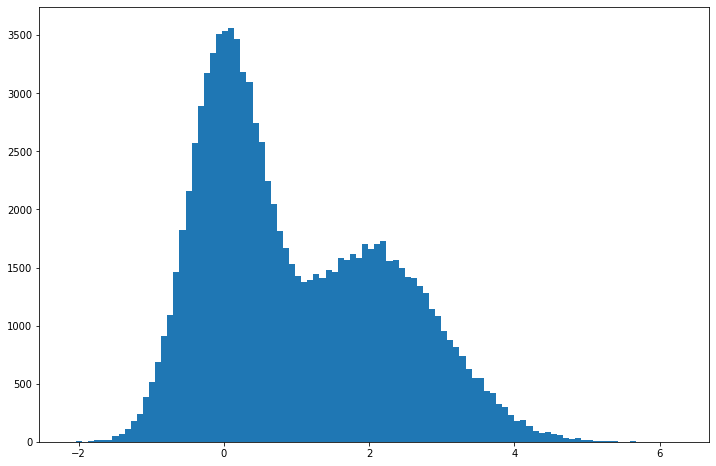
\includegraphics[width=0.7\linewidth]{./gaussian_mixture_1.png}
\end{textblock*}
\end{frame}



\begin{frame}{正規分布の再生性}
\begin{itemize}
\item $M$個の確率変数$x_1,\ldots,x_M$が、それぞれ独立に正規分布$\mathcal{N}(\mu_1,\sigma_1^2), 
\ldots, \mathcal{N}(\mu_M,\sigma_M^2)$にしたがうとする。
\item このとき、$\sum_{m=1}^M a_m x_m$は、以下の正規分布にしたがう:
\begin{align}
\mathcal{N}(\sum_m a_m \mu_m, \sum_m a_m^2 \sigma_m^2)
\end{align}
\end{itemize}
\end{frame}

\section{単変量正規分布の最尤推定}

\begin{frame}\frametitle{Contents}
\Large \tableofcontents[currentsection]
\end{frame}

\begin{frame}{単変量正規分布に従う観測データの尤度}
\begin{itemize}
\item 与えられている観測データを$\mathcal{D}=\{x_1,\ldots,x_N\}$とする
\begin{itemize}
\item 各$x_i$は、$-\infty < x_i < \infty$を満たす実数値とする
\end{itemize}
\item 各$x_i$は同じ正規分布$\mathcal{N}(\mu,\sigma)$に独立にしたがうものとして、この観測データをモデル化することにする
\item このときデータセット$\mathcal{D}$の尤度は、以下のような$\mu$と$\sigma$の関数になる
\begin{align}
p(\mathcal{D};\mu,\sigma)=\prod_{i=1}^N p(x_i;\mu,\sigma)
=\prod_{i=1}^N \frac{1}{\sqrt{2\pi\sigma^2}}\exp\bigg( - \frac{(x_i - \mu)^2}{2\sigma^2}\bigg)
\end{align}
\end{itemize}
\end{frame}


\begin{frame}{単変量正規分布の最尤推定}
\begin{itemize}
\item よって、観測データ$\mathcal{D}$の対数尤度は以下のようになる
\begin{align}
\ln p(\mathcal{D};\mu,\sigma)
= -\frac{N}{2}\ln(2\pi\sigma^2) - \sum_{i=1}^N \frac{(x_i - \mu)^2}{2\sigma^2}
\end{align}
\item この対数尤度を最大化する$\mu$と$\sigma$を、以下、求める
\end{itemize}
\end{frame}


\begin{frame}
\begin{align}
\frac{\partial \ln p(\mathcal{D};\mu,\sigma)}{\partial \mu}
= \sum_{i=1}^N \frac{x_i - \mu}{\sigma^2}
\end{align}
$\frac{\partial \ln p(\mathcal{D};\mu,\sigma)}{\partial \mu}=0$より
$\mu = \frac{\sum_i x_i}{N} = \bar{x}$(標本平均)
\begin{align}
\frac{\partial \ln p(\mathcal{D};\mu,\sigma)}{\partial \sigma}
= - \frac{N}{\sigma} + \sum_{i=1}^N \frac{(x_i - \mu)^2}{\sigma^3}
\end{align}
$\frac{\partial \ln p(\mathcal{D};\mu,\sigma)}{\partial \sigma} = 0$より
$\sigma^2 = \frac{\sum_i (x_i - \mu)^2}{N} = \frac{\sum_i (x_i - \bar{x})^2}{N}$(標本分散)
\end{frame}

%\begin{frame}{分散の推定値}
%\begin{itemize}
%\item 最尤推定で求まる分散の推定値は、不偏分散とは異なる
%\item 最尤推定で求まったのは、標本分散
%\item 標本分散の期待値は、母分散に一致しない
%\item 不偏分散(下の式)の期待値は、母分散に一致する
%\begin{align}
%\hat{\sigma}^2 = \frac{1}{N - 1}\sum_{i=1}^N \frac{(x_i - \bar{x})^2}{N}
%\end{align}
%\end{itemize}
%\end{frame}

\section{多変量正規分布}

\begin{frame}\frametitle{Contents}
\Large \tableofcontents[currentsection]
\end{frame}

\begin{frame}{二変量正規分布}
\begin{itemize}
\item パラメータ
\begin{itemize}
\item 平均ベクトル
$\bm{\mu} = \begin{bmatrix} \mu_1 \\ \mu_2 \end{bmatrix}$
\item 分散共分散行列
$\bm{\Sigma} = \begin{bmatrix} \sigma_{11} & \sigma_{12} \\ \sigma_{12} & \sigma_{22} \end{bmatrix}$
(ただし$\Sigma$は正定値行列)
\end{itemize}
\item 確率密度関数(ただし$| \bm{\Sigma} | \equiv \mbox{det}\bm{\Sigma}$)
\begin{align}
p(\bm{x};\bm{\mu},\bm{\Sigma}) = \frac{1}{\sqrt{(2\pi)^2|\bm{\Sigma}|}}\exp\bigg\{ - \frac{(\bm{x} - \bm{\mu})^\intercal \bm{\Sigma}^{-1} (\bm{x} - \bm{\mu})}{2} \bigg\}
\end{align}
\end{itemize}
\end{frame}

\begin{frame}{多変量正規分布}
\begin{itemize}
\item パラメータ
\begin{itemize}
\item 平均ベクトル
$\bm{\mu} = \begin{bmatrix} \mu_1 \\ \vdots \\ \mu_d \end{bmatrix}$
\item 分散共分散行列
$\bm{\Sigma} = \begin{bmatrix} \sigma_{11} & \cdots & \sigma_{1d} \\ 
\vdots & \ddots & \vdots \\
\sigma_{1d} & \cdots & \sigma_{dd} \end{bmatrix}$
(ただし$\Sigma$は正定値行列)
\end{itemize}
\item 確率密度関数(ただし$| \bm{\Sigma} | \equiv \mbox{det}\bm{\Sigma}$)
\begin{align}
p(\bm{x};\bm{\mu},\bm{\Sigma}) = \frac{1}{\sqrt{(2\pi)^d|\bm{\Sigma}|}}\exp\bigg\{ - \frac{(\bm{x} - \bm{\mu})^\intercal \bm{\Sigma}^{-1} (\bm{x} -\bm{\mu})}{2} \bigg\}
\end{align}
\end{itemize}
\end{frame}

\begin{frame}{共分散行列 covariance matrix}
\begin{itemize}
\item 二変量以上の場合、2つ以上成分をもつベクトルをモデル化
\item ベクトルの第1成分、第2成分、等々について、各々単独での散らばり方は、当然考慮する
\begin{itemize}
\item これが、共分散行列の対角成分、つまり分散に対応する
\end{itemize}
\item これに加えて、第1成分と第2成分、第1成分と第3成分など、異なる成分間の関連も考慮する
\begin{itemize}
\item これが、共分散行列の非対角成分、つまり共分散に対応する
\end{itemize}
\item 共分散行列は分散共分散行列とも呼ばれる
\end{itemize}
\end{frame}

\begin{frame}{共分散covarianceの直感的な意味}
\begin{itemize}
\item 共分散は共分散行列の非対角成分に現れている値
\item ゼロだと、対応する二つの成分は独立に分布
\item 正の値だと、一方の成分が平均より大きいとき、他方の成分も平均より大きくなることが多い
\item 負の値だと、一方の成分が平均より大きいとき、他方の成分は平均より小さくなることが多い
\end{itemize}
\end{frame}

\begin{frame}
\begin{figure}[t]
\begin{center}
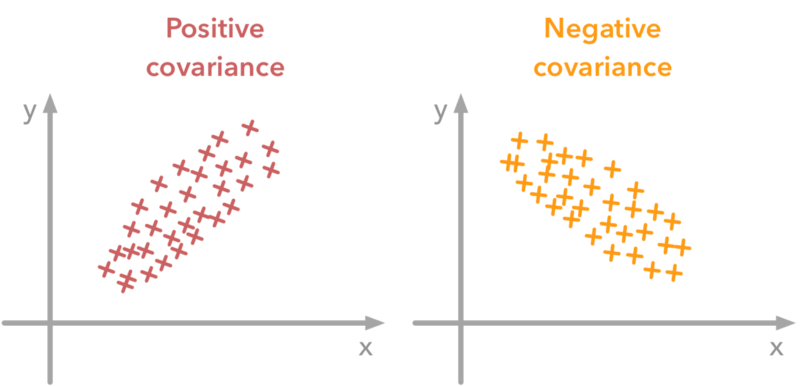
\includegraphics[scale=0.5]{1_GH0ou22oJEwAw89GkrS8-w.png}
\href{https://www.kdnuggets.com/2018/10/preprocessing-deep-learning-covariance-matrix-image-whitening.html}{\tiny\url{https://www.kdnuggets.com/2018/10/preprocessing-deep-learning-covariance-matrix-image-whitening.html}}
\label{}
\end{center}
\end{figure}
\end{frame}

\begin{frame}
\begin{columns}[c,onlytextwidth]
\begin{column}{.3\textwidth}
$\bm{\mu} = \begin{bmatrix} 0 \\ 1 \end{bmatrix}$

$\bm{\Sigma} = \begin{bmatrix} 1 & -0.5 \\ -0.5 & 1.5 \end{bmatrix}$
\end{column}
\begin{column}{.7\textwidth}
\begin{figure}[c]
\begin{center}
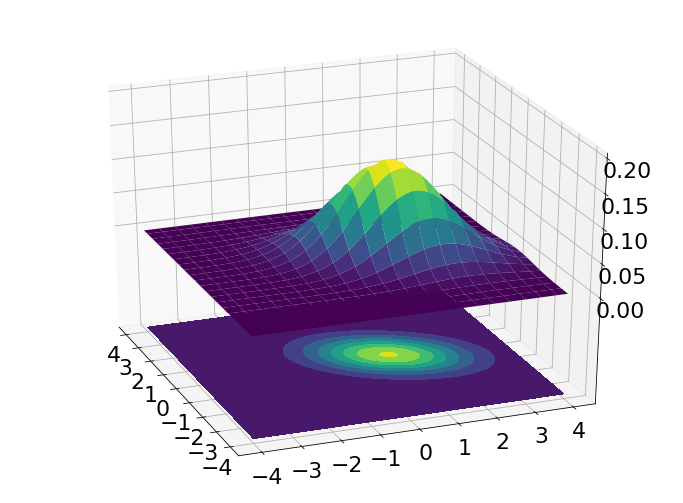
\includegraphics[scale=0.4]{normal_distribution_3.png}
\end{center}
\caption{二変量正規分布の密度関数の例}
\end{figure}
\end{column}
\end{columns}
\end{frame}

\begin{frame}{問題4-1}
\begin{itemize}
\item $\bm{\Sigma} = \begin{bmatrix} 1 & -1 \\ -1 & 2 \end{bmatrix}$の行列式$\mbox{det}\bm{\Sigma}$を求めよ。
\item $\bm{\Sigma} = \begin{bmatrix} 1 & -1 \\ -1 & 2 \end{bmatrix}$の逆行列$\bm{\Sigma}^{-1}$を求めよ。
\end{itemize}
\end{frame}

\begin{frame}{二変量正規分布の別のパラメータ化(1/2)}
\begin{itemize}
\item 同じ確率分布でも、パラメータ化parameterizationの方法が複数あることがある
\item 二変量正規分布では、共分散行列を以下のようにパラメータ化することがある
\begin{itemize}
\item 自由度は3で変わらないことに注意
\end{itemize}
\end{itemize}
\begin{align}
\bm{\Sigma} = \begin{bmatrix} \sigma_1^2 & \rho\sigma_1\sigma_2 \\
\rho\sigma_1\sigma_2 & \sigma_2^2 \end{bmatrix}
\end{align}
\end{frame}

\begin{frame}{二変量正規分布の別のパラメータ化(2/2)}
\begin{itemize}
\item このパラメータ化のもとでは$\bm{\Sigma}$の行列式と逆行列は
\end{itemize}
\begin{align}
\mbox{det}\bm{\Sigma} &= \sigma_1^2\sigma_2^2(1-\rho^2) \\
\bm{\Sigma}^{-1} &= \frac{1}{\mbox{det}\bm{\Sigma}}
\begin{bmatrix} \sigma_2^2 & -\rho\sigma_1\sigma_2 \\ -\rho\sigma_1\sigma_2 & \sigma_1^2 \end{bmatrix}
\end{align}
\end{frame}

\section{多変量正規分布の最尤推定}

\begin{frame}\frametitle{Contents}
\Large \tableofcontents[currentsection]
\end{frame}

\begin{frame}{多変量正規分布の最尤推定}
\begin{itemize}
\item 観測データ$\mathcal{D}=\{ \bm{x}_1,\ldots,\bm{x}_N\}$の各$\bm{x}_i$が独立に同じ正規分布$\mathcal{N}(\bm{\mu},\bm{\Sigma})$にしたがうと仮定すると、$\mathcal{D}$の尤度は:
\begin{align}
& p(\mathcal{D};\bm{\mu},\bm{\Sigma})
= \prod_{i=1}^N p(\bm{x}_i;\bm{\mu},\bm{\Sigma})
\notag \\ & =
\prod_{i=1}^N \frac{1}{\sqrt{(2\pi)^d|\bm{\Sigma}|}}
\exp\bigg( - \frac{1}{2} (\bm{x}_i - \bm{\mu})^\intercal \bm{\Sigma}^{-1} (\bm{x}_i - \bm{\mu}) \bigg)
\end{align}
\item 最尤推定によって各パラメータを推定(次スライドから)
\end{itemize}
\end{frame}

\begin{frame}{行列やベクトルの偏微分の基本を再確認}
\vspace{-.3in}
\begin{align}
\frac{\partial x_{kl}}{\partial x_{ij}} & = \delta_{ik} \delta_{lj}\\
& \mbox{ ただし、$i=k$ならば$\delta_{ik}=1$、そうでなければ$\delta_{ik}=0$} \notag \\
\bigg[ \frac{\partial \bm{x}}{\partial y} \bigg]_i & = \frac{\partial x_i}{\partial y} \\
\bigg[ \frac{\partial x}{\partial \bm{y}} \bigg]_i & = \frac{\partial x}{\partial y_i} \\
\bigg[ \frac{\partial \bm{x}}{\partial \bm{y}} \bigg]_{ij} & = \frac{\partial x_i}{\partial y_j} 
\end{align}
\end{frame}

\begin{frame}
\FontMath
\begin{align}
& \ln p(\mathcal{D};\bm{\mu},\bm{\Sigma}) =\sum_{i=1}^N \ln p(\bm{x}_i;\bm{\mu},\bm{\Sigma}) \notag \\
& = - \frac{Nd}{2}\ln(2\pi) - \frac{N}{2}\ln(|\bm{\Sigma}|) - \frac{1}{2}\sum_i
(\bm{x}_i - \bm{\mu})^\intercal \bm{\Sigma}^{-1} (\bm{x}_i - \bm{\mu})
\end{align}
ここで、$\bar{\bm{x}}=\frac{\sum_i \bm{x}_i}{N}$として、
\begin{align}
\sum_i (\bm{x}_i - \bm{\mu})^\intercal \bm{\Sigma}^{-1} (\bm{x}_i - \bm{\mu})
= \sum_i \bm{x}_i^\intercal\bm{\Sigma}^{-1}\bm{x}_i 
- 2N\bar{\bm{x}}^\intercal\bm{\Sigma}^{-1}\bm{\mu}
+ N\bm{\nu}^\intercal\bm{\Sigma}^{-1}\bm{\mu}
\end{align}
より、
\begin{align}
\frac{\partial \ln p(\mathcal{D};\bm{\mu},\bm{\Sigma})}{\partial \bm{\mu}}
& = - N \bm{\Sigma}^{-1} \bar{\bm{x}} + N \bm{\Sigma}^{-1}\bm{\mu} \\
\therefore \bm{\mu} & = \bar{\bm{x}}
\end{align}
\end{frame}

\begin{frame}
\FontMath
$\frac{\partial \ln p(\mathcal{D};\bm{\mu},\bm{\Sigma})}{\partial \bm{\Sigma}}$の計算は、
\href{https://www.ics.uci.edu/~welling/teaching/KernelsICS273B/MatrixCookBook.pdf}{The Matrix Cookbook}を見ながらおこなう。
\begin{align}
\frac{\partial}{\partial \bm{\Sigma}}\ln(|\bm{\Sigma}|) & = \bm{\Sigma}^{-1} \\
\frac{\partial}{\partial \bm{\Sigma}}
(\bm{x}_i - \bm{\mu})^\intercal \bm{\Sigma}^{-1} (\bm{x}_i - \bm{\mu})
& = - \bm{\Sigma}^{-1} (\bm{x}_i - \bm{\mu}) (\bm{x}_i - \bm{\mu})^\intercal \bm{\Sigma}^{-1}
\end{align}
以上より、
\begin{align}
\frac{\partial \ln p(\mathcal{D};\bm{\mu},\bm{\Sigma})}{\partial \bm{\Sigma}}
&= - \frac{N}{2}\bm{\Sigma}^{-1}
+ \frac{1}{2} \bm{\Sigma}^{-1}  \bigg( \sum_i
(\bm{x}_i - \bm{\mu}) (\bm{x}_i - \bm{\mu})^\intercal \bm{\Sigma}^{-1} \bigg) \bm{\Sigma}^{-1} \notag \\
&= - \frac{1}{2}\bm{\Sigma}^{-1} \bigg\{
N - \bigg( \sum_i
(\bm{x}_i - \bm{\mu}) (\bm{x}_i - \bm{\mu})^\intercal \bm{\Sigma}^{-1} \bigg) \bm{\Sigma}^{-1} \bigg\} \\
\therefore
\bm{\Sigma} &= \frac{1}{N}\sum_i
(\bm{x}_i - \bm{\mu}) (\bm{x}_i - \bm{\mu})^\intercal 
\end{align}
\end{frame}

\section{多変量正規分布の最尤推定の応用}

\begin{frame}\frametitle{Contents}
\Large \tableofcontents[currentsection]
\end{frame}

\begin{frame}
\begin{figure}[htbp]
\begin{center}

\includegraphics[scale=.45]{book_anomaly.png}
\end{center}
\end{figure}
\end{frame}

\begin{frame}{異常検知への応用:ホテリングの$T^2$法の概要}
\begin{itemize}
\item 異常値を含まない(あるいはほとんど含まない)データ集合を使って多変量正規分布のパラメータを最尤推定する
\item 異常値かどうかを調べたいデータについて、最尤推定の結果を使って標本平均とのマハラノビス距離を求める
\item マハラノビス距離が、あらかじめ計算しておいた閾値を超えたとき、警報を出す
\end{itemize}
\end{frame}

\begin{frame}{観測データの異常度}
\begin{itemize}
\item 最尤推定で求めた平均ベクトルを$\hat{\bm{\mu}}$、共分散行列を$\hat{\bm{\Sigma}}$とする
\item この推定値を使うと正規分布の密度関数は
\begin{align}
p(\bm{x};\hat{\bm{\mu}},\hat{\bm{\Sigma}}) = 
\frac{1}{\sqrt{(2\pi)^d|\hat{\bm{\Sigma}}|}} \exp \bigg\{
- \frac{1}{2} (\bm{x} - \hat{\bm{\mu}})^\intercal \hat{\bm{\Sigma}}^{-1}
(\bm{x} - \hat{\bm{\mu}}) \bigg\}
\end{align}
\item そして、観測データ$\bm{x}$の異常度を$-\ln p(\bm{x};\hat{\bm{\mu}},\hat{\bm{\Sigma}})$と定義する
\begin{itemize}
\item 直感的には、推定された平均ベクトル$\hat{\bm{\mu}}$から遠いほど異常
\item ただし、ユークリッド距離を使っているのではない
\end{itemize}
\end{itemize}
\end{frame}

\begin{frame}{マハラノビス距離 Mahalanobis distance}
\begin{itemize}
\item 異常度$-\ln p(\bm{x};\hat{\bm{\mu}},\hat{\bm{\Sigma}})$から定数部分を除いたものを、
$\bm{x}$の$\hat{\bm{\mu}}$からのマハラノビス距離という
\item $\bm{x}$の$\hat{\bm{\mu}}$からのマハラノビス距離を$\alpha(\bm{x})$と書くことにすると
\begin{align}
\alpha(\bm{x}) = (\bm{x} - \hat{\bm{\mu}})^\intercal \hat{\bm{\Sigma}}^{-1}
(\bm{x} - \hat{\bm{\mu}})
\end{align}
\item $\alpha(\bm{x})$が大きいほど$\bm{x}$はより一層異常とみなす
\begin{itemize}
\item $\hat{\bm{\Sigma}}$を使っているので、観測データのベクトルの成分間の関連も考慮した距離になっている
\end{itemize}
\end{itemize}
\end{frame}

\begin{frame}{ホテリングの$T^2$法}
\begin{itemize}
\item 同じ$d$次元正規分布$\mathcal{N}(\bm{\mu},\bm{\Sigma})$からの$N$個の独立なサンプルだと仮定された観測データに基づき、最尤推定により平均ベクトルを$\hat{\bm{\mu}}$、共分散行列を$\hat{\bm{\Sigma}}$と、それぞれ推定したとする
\item このとき、$T^2 \equiv \frac{N-d}{(N+1)d}a(\bm{x})$により定義される統計量$T^2$は、自由度$(d,N-d)$のF分布にしたがう
\item $N \gg d$の場合は、$a(\bm{x})$は近似的に自由度$d$のカイ2乗分布にしたがう
\end{itemize}
\end{frame}

\begin{frame}{カイ2乗分布}
\begin{itemize}
\item 独立に標準正規分布にしたがう$k$個の確率変数の二乗和がしたがう分布を、自由度$k$のカイ2乗分布とよぶ
\end{itemize}
\begin{figure}[htbp]
\begin{center}
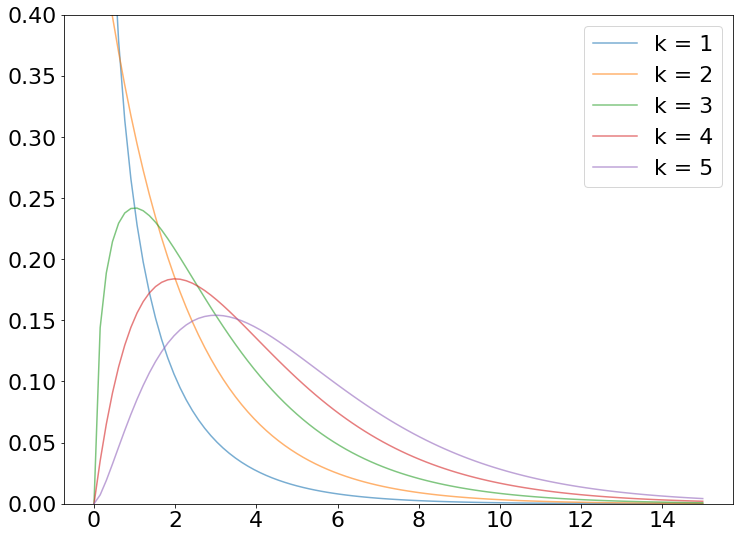
\includegraphics[scale=.3]{chi2.png}
\end{center}
\end{figure}
\end{frame}

\begin{frame}{閾値の決め方}
\begin{columns}[onlytextwidth]
\begin{column}{.6\textwidth}
\begin{itemize}
\item あらかじめ誤報率$\alpha$を決めておく
\item 下の等式を満たすようにマハラノビス距離の閾値$a_0$を決める
\begin{align}
1 - \alpha = \int_0^{a_0} \chi^2(x;d) dx
\end{align}
\item ただし、$\chi^2(x;d)$は自由度$d$のカイ2乗分布の確率密度関数とする
\end{itemize}
\end{column}
\begin{column}{.4\textwidth}
\begin{figure}[htbp]
\begin{center}
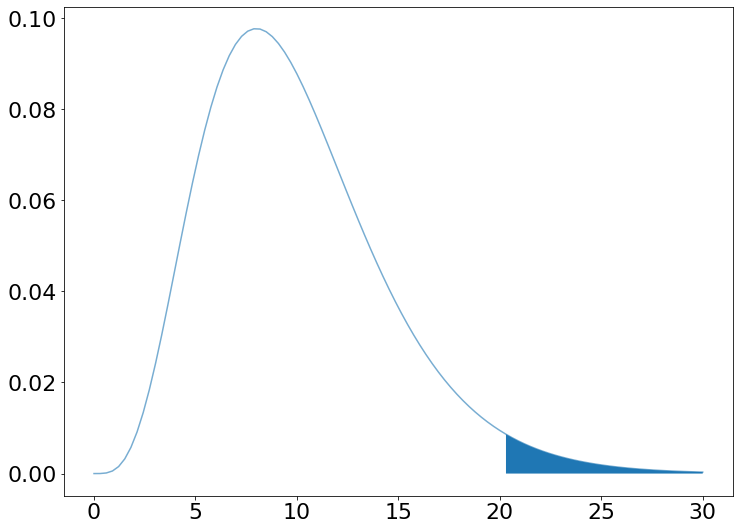
\includegraphics[scale=.25]{chi2_2.png}
\end{center}
\end{figure}
\end{column}
\end{columns}
\end{frame}

\end{document}
